\section{Problema 2: Alta Frecuencia}
\subsection{Descripci\'on de la problem\'atica}

Se quiere transmitir informaci\'on secuencialmente mediante un enlace el mayor tiempo posible. Los enlaces tienen asociadas distintas frecuencias, con un costo por minuto y un intervalo de tiempo (sin cortes) en el cual funcionan. Se utilizan durante minutos enteros, y es posible cambiar de una frecuencia a otra instant\'anemente (del minuto 1 al 4 uso la frecuencia A y del 4 al 6 la B). Los datos del precio y e intervalo de tiempo de cada frecuencia son dados. Se desea optimizar este problema para transmitir todo el tiempo que tenga al menos una frecuencia abierta, pero gastando la menor cantidad de dinero. Se debe contar con una complejidad de $O(n.log(n))$.\\

A continuaci\'on se muestran dos casos particulares de este problema. En ambos se ofrecen tres frecuencias, con distintos costos cada una. Se puede ver recuadrado en violeta cu\'al es la elecci\'on que debe hacerse por intervalo de tiempo.


 \begin{figure}[h!]
   \begin{center}
 	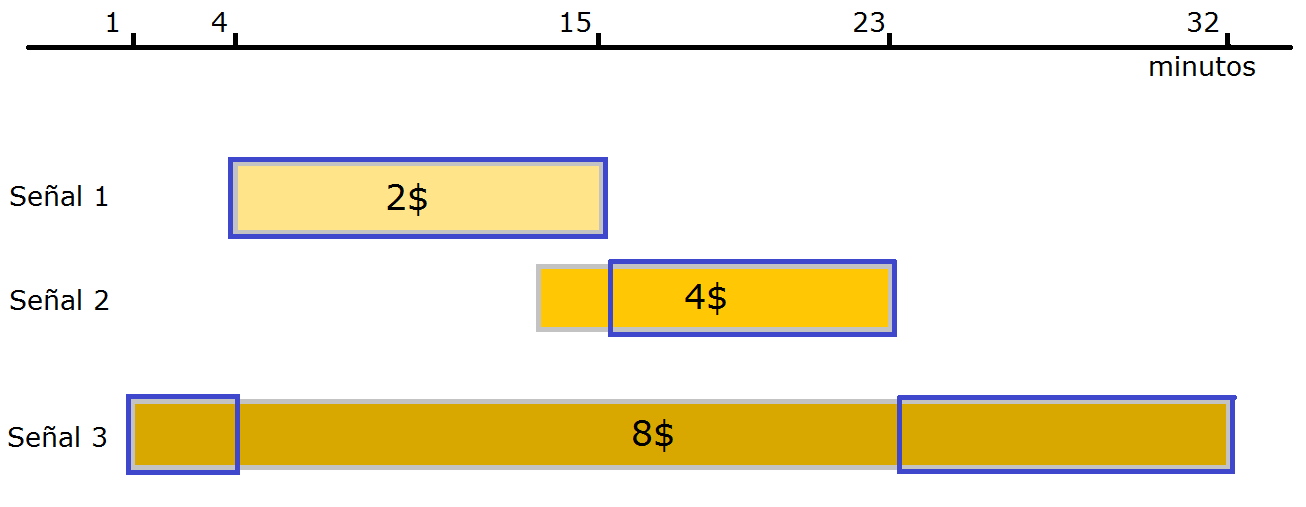
\includegraphics[scale=0.45]{imagenes/ej2/ejemplo1.png}
 	\caption{Ejemplo 1}
% 	\label{caballito}	
   \end{center}
 \end{figure}

 \begin{figure}[h!]
   \begin{center}
 	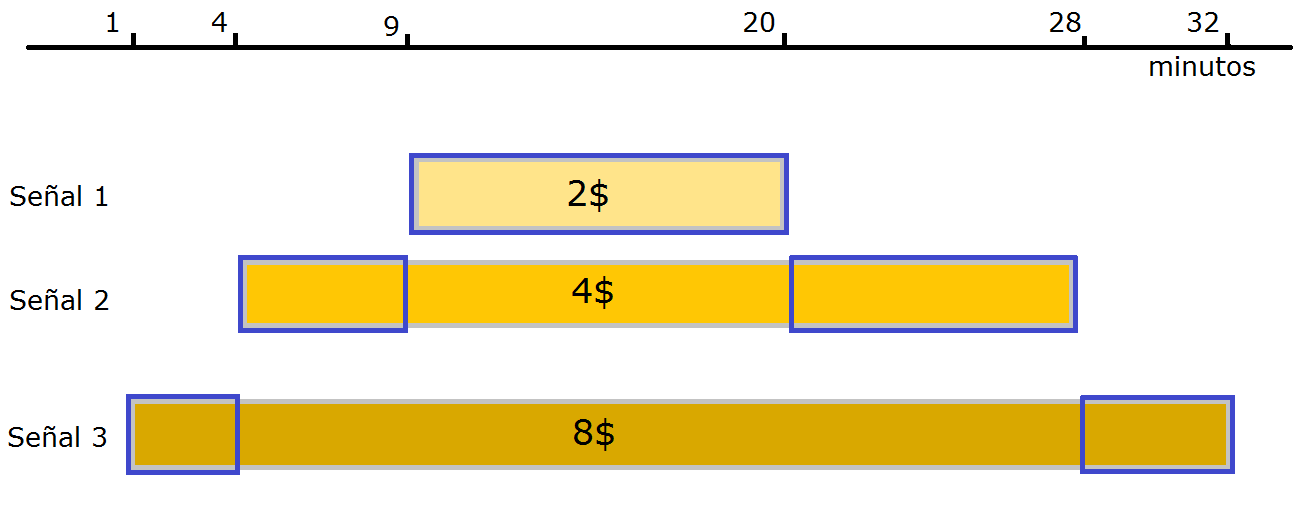
\includegraphics[scale=0.45]{imagenes/ej2/ejemplo2.png}
 	\caption{Ejemplo 2}
% 	\label{caballito}	
   \end{center}
 \end{figure}


\newpage

\subsection{Resoluci\'on propuesta y justificaci\'on}

El algoritmo que utilizamos pertenece a la familia de \emph{Divide \& Conquer}.\\

\textcolor{red}{Aca pasa lo mismo de la implementacion porque hablamos mucho de vector y bla...}\\

Todas las frecuencias se encuentran almacenadas en un vector. Primero se las ordena en orden creciente respecto del costo, es decir en la primera posición se almacena la m\'as barata y en la última, la más cara. Una vez que contamos con este ordenamiento inicial, se va a proseguir mediante el \emph{divide} dentro de este vector.\\

Se prosigue de acuerdo a las características de Divide \& Conquer. De modo recursivo, se divide al vector pasado por parámetro por la mitad creando dos nuevos a los cuales se les aplica nuestro algoritmo de merge. El caso base se da cuando el vector tiene un sólo elemento, para lo cual se devuelve el vector tal cual entró.

	\begin{codesnippet}
	\begin{verbatim}
divide(conjuntoDeFrecuencias F){
    Si hay mas de un elemento:
        Divido F en dos conjuntos A, B.
        divide(A)
        divide(B)
        Devuelvo conquer(A,B)
    Si hay un solo elemento:
        Lo devuelvo.	
}
	\end{verbatim}
	\end{codesnippet}

Nuestro algoritmo de Merge (\emph{conquer}) se encarga de elegir entre las frecuencias de dos arreglos pasados como parámetro, de modo que devuelve un sólo vector indicando los intervalos ocupados por las frecuencias elegidas. 

Dado el enunciado del problema, para elegir qu\'e frecuencia utilizar en determinado intervalo de tiempo se debe priorizar el precio más barato emitiendo señal siempre que sea posible. Gracias a que en el primer llamado de nuestra funci\'on estas se encontraban en orden creciente respecto del costo, en cada paso de \emph{merge} de los dos arreglos de entrada con intervalos se van a priorizar los de la izquierda. Es decir que en cada paso, todos los intervalos pertenecientes al vector de la izquierda (como son los de menor precio) van a pertencer al vector resultado. Mientras que s\'olo los intervalos que completen tiempo sin se\~nal pertenecientes al vector de la derecha van a ser colocados en el vector resultado. Esto representa un invariante que se va a cumplir en cada paso del algoritmo, lo cual nos permite justificar que la soluci\'on obtenida es la deseada. \textcolor{red}{Que alguien lea esto para ver si se entiende, para mi si :)}\\

	\begin{codesnippet}
	\begin{verbatim}
conquer(conjuntoDeFrecuencias A, conjuntoDeFrecuencias B){
	vector<frecuencia>::iterator iterCara = cara.begin(), iterBarata = barata.begin();
	vector<frecuencia> res;
	
	En el conjunto res voy a tener el resultado.
    Voy recorriendo en orden A y B, mientras haya elementos en A:
    //Llamo A[i] al intervalo actual de A y B[j] al de B.
        Si B[j] comienza antes que A[i]:
            Si B[j] termina antes que A[i]:
                Inserto B[j] en res.
                j++
            Si B[j] termina despues que A[i] empiece                                                                                                                                                                                                                                                                                                                                                                                                                                                                                                                                                                                                                                                                                                                                                                                                                                                                                                                                                                                                                                                                                                                                                                                                                                                                                                                                                              :
                
    
    
        Si A[i] comienza antes que B[j]:
            Inserto A[i] en res
            Si B[j] se superpone en algun momento con A[i]:
                Al comienzo de B[j] le asigno el final de A[i]




	while(iterCara != cara.end()){
		if(iterBarata != barata.end()){
			if(iterCara->principio < iterBarata->principio){ //la cara empieza antes
				if(iterCara->fin <= iterBarata->principio){ //la cara termina antes de que empiece la barata
					res.push_back(*iterCara);				//meto la cara entera
					iterCara++;
				}
				else{ //la cara empieza antes y termina despues del principio de la barata
					frecuencia antes;
					antes.id = iterCara->id;
					antes.costo = iterCara->costo;
					antes.principio = iterCara->principio;
					antes.fin = iterBarata->principio;
					res.push_back(antes);
					iterCara->principio = iterBarata->fin;
				}
			}
			else{ //la barata empieza antes (o igual) que la cara
				if(iterCara->fin > iterBarata->fin){ //la cara termina despues que la barata
					if (iterCara->principio < iterBarata->fin) //este if es nuevo
						iterCara->principio = iterBarata->fin;
					res.push_back(*iterBarata);
					iterBarata++;
				}
				else
					iterCara++;
			}
		}
		else{
			if(iterCara->principio < iterCara->fin)
				res.push_back(*iterCara);
			iterCara++;
		}
	}
	while(iterBarata != barata.end()){
		res.push_back(*iterBarata);
		iterBarata++;
	}
	return res;
}

	\end{verbatim}
	\end{codesnippet}






Este algoritmo resuelve lo propuesto dando una soluci\'on \'optima porque del modo en que est\'a definido, primero divide al grupo con todas las frecuencias ofrecidas recursivamente hasta llegar a conjuntos con una sola frecuencia. Luego, al momento de mergear estos grupos de a dos, siempre prioriza al grupo de la izquierda (el m\'as barato). 

Esto quiere decir que en el primer paso de este \textit{merge} se van a comparar solamente dos frecuencias entre s\'i, colocando la frecuencia m\'as barata completa y; si la oferta de intervalos de la frecuencia m\'as cara completa uno o dos intervalos donde no se le hab\'ia asignado se\~nal, se le otorga a ellos la frecuencia m\'as cara. De este modo, comparamos de a dos, frecuencias consecutivas otorg\'andole prioridad a la frecuencia m\'as barata. \textcolor{red}{Poner dibujito.} 

En el siguiente paso del \textit{merge} se van a comparar dos conjuntos de intervalos con dos frecuencias en cada uno. Cada uno de estos conjuntos puede estar conformado por uno, dos o tres intervalos. \textcolor{red}{Poner dibujito} Gracias al formato de nuestro algoritmo, en cada paso del merge se preserva el invariante de que el conjunto ubicado a la izquierda tiene las frecuencias m\'as baratas mientras que el de la derecha tiene las m\'as caras. Se prosigue de manera an\'aloga a lo anterior, se preservan todos los intervalos de frecuencias pertenecientes al conjunto de los m\'as baratos y s\'olo se agregan frecuencias del conjunto caro en caso de que esten disponibles en intervalos de tiempos que hayan quedado vac\'ios.

Estos pasos se van a reiterar, comparando conjuntos de intervalos entre dos, hasta que se hayan recorrido todas las frecuencias.\\


Una vez terminados todos los pasos recursivos, vamos a contar con el conjunto de intervalos que completen la mayor cantidad de tiempo con el costo m\'as bajo. Si no hay dos frecuencias con el mismo costo, esta soluci\'on (\'optima) es \'unica, en caso contrario podr\'ia existir m\'as de una soluci\'on \'optima. \\



\newpage

\subsection{An\'alisis de la complejidad}

Primero consideramos que nos encontramos en un caso donde la soluci\'on \'optima es \'unica. Si contamos con la oferta de \emph{n} frecuencias, podemos asegurar que la cantidad de intervalos que va a contener la salida es de, a lo sumo, \emph{2n-1}. Esta cota superior est\'a dada porque, si consideramos agregar de a una las distintas frecuencias (empezando por las de menor costo), lo m\'aximo que puede agregar son dos intervalos (o cubrir huecos de otros que no llegaron a llenar dos). \textcolor{red}{Aca viene Eze y explica bien todo esto :D}.

Por lo tanto, al hacer nuestro algoritmo de Divide \& Conquer vamos a contar con, a lo sumo, 2n-1 intervalos. Esto nos otorga una complejidad de \emph{O(n.log(n))} por el Teorema de ??????.

\newpage
\subsection{C\'odigo fuente}
\newpage
\subsection{Experimentaci\'on}

\subsubsection{Constrastaci\'on Emp\'irica de la complejidad}
-Comparar tiempos para 10, 100, 1000, 10000 y 100000 intervalos generando aleatoriamente varios de cada una y scar promedio. Hacer lo que hicieron en clase\\


\newpage
\subsubsection{Modificaci\'on del algoritmo}
Debido a que nuestro algoritmo no considera como caso espec\'ifico el ordenar distintas frecuencias con el mismo valor, al momento de elegir intervalos se podr\'ian realizar cortes innecesario. Es decir, no siempre se elige la cantidad m\'inima posible en estos casos.\\

Como consideramos que esto puede tardar un tiempo no despreciable, modificamos el operador $<$ para frecuencias, de modo que cuando tiene dos frecuencias del mismo valor ingrese primero la que tenga el comienzo antes y, en caso de comenzar en simult\'aneo, ingrese primero la frecuencia de mayor tama\~no.\\

\textcolor{red}{Aca poner el codigo que se deberia modificar.}\\

\textcolor{red}{Aca va el grafico de esto}\\

\textcolor{red}{Comentar si paso lo que esperabamos o no.}
